\documentclass[]{article}
\usepackage{caption,subcaption,graphicx,float,url,amsmath,amssymb,amsthm,tocloft,cancel,thmtools,gensymb,braket}
\usepackage[toc,nonumberlist]{glossaries}
\usepackage{glossaries-extra}
\usepackage[toc,page]{appendix}

\newcommand\numberthis{\addtocounter{equation}{1}\tag{\theequation}}

\newtheorem{thm}{Theorem}
\newtheorem{defn}[thm]{Definition}
\newtheorem{cor}[thm]{Corollary}
\newtheorem{lemma}[thm]{Lemma}
\graphicspath{{figs/}}
\widowpenalty10000
\clubpenalty10000
\setcounter{tocdepth}{2}

%opening
\title{Theoretical Minimum\\Particle Physics 2\\Standard Model}
\author{Simon Crase(compiler)}

\begin{document}

\maketitle

\begin{abstract}
These are my notes for the \emph{New Revolutions in Particle Physics 2} lectures from Leonard Susskind's \emph{Theoretical Minimum} series\cite{susskind2009standard}. Since this material predates the discovery of the Higgs Boson, there is an appendix \emph{Demystifying the Higgs Boson} \cite{susskind2010demystifing}.
\end{abstract}

\tableofcontents
\listoffigures
\listoftables
\listoftheorems

\section{Particles fields and forces}

Figure \ref{fig:particles:fields:forces} shows a triangle of concepts:
\begin{itemize}
	\item particles (quanta of fundamental fields)\footnote{We are going to have to think very hard about what is an elementary particles and what is composite always be frustrated, always find some slippery region why your definition did not work.}
	\item Fields
	\item Forces
\end{itemize}

\begin{figure}[H]
	\begin{center}
		\caption{Triangle of concepts: particles, fields, and forces}\label{fig:particles:fields:forces}
		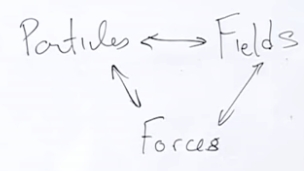
\includegraphics[width=0.5\textwidth]{ParticlesFieldsForces}
	\end{center}
\end{figure}

Consider two electric charges

\begin{align*}
E=&\int (e_1 \vec{E_1})^2 dV\\
E=&\int (e_2 \vec{E_2})^2 dV\\
E=&\int (e_1\vec{E_1}+e_2 \vec{E_2})^2 dV\\
=&\int \underbrace{(e_1\vec{E_1})^2}_\text{self energy}+ \underbrace{(e_2\vec{E_2})^2}_\text{self energy} + \underbrace{2e_1e_2\vec{E_1}.\vec{E_2}}_\text{interesting term}
\end{align*}

The first two terms represent self energy, which is includes in mass; the last term is proportional to the charges.
\begin{itemize}
	\item  If they are so far away that $\vec{E_1}$ is negligible near second charge there will be no perceptible effect.
	\item If the particles are close we will get a contribution from $\vec{E_1}.\vec{E_2}$. This turns out to be the Coulumb force. 
\end{itemize}

The force comes from the distortion of the field: this is a \emph{purely field view of forces}. If fields give rise to forces, and particles are quanta of fields, there must be a way to think of forces coming from particles.

Where do molecular forces come from? There are several mechanisms: we will focus on one. Imagine two protons and a single electron. Electron hops because of tennelling. \footnote{Don't watch tunnelling! Like any QM effect, watching ruins it.}

\begin{figure}[H]
	\caption[Molecular forces: two protons and a single electron]{Two protons and a single electron. Classically electron can't swap between Figures \ref{fig:2proton1Electrona} and \ref{fig:2proton1Electronb}, but QM allows it to tunnel.}
	\begin{subfigure}{0.45\textwidth}
		\caption{Right hand protons is a long way from Left: Schr\"odinger wave function for electron near left hand.} 
		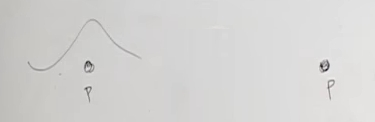
\includegraphics[width=0.9\textwidth]{2proton1Electrona}\label{fig:2proton1Electrona}
	\end{subfigure}
	\begin{subfigure}{0.45\textwidth}
		\caption{Protons closer together: Figure \ref{fig:2proton1Electrona} still possible, but so is this--same energy.}
		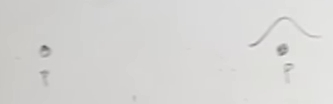
\includegraphics[width=0.9\textwidth]{2proton1Electronb}\label{fig:2proton1Electronb}
	\end{subfigure}
	\begin{subfigure}{0.45\textwidth}
		\caption{Effect of tunnelling}
		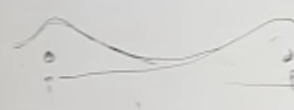
\includegraphics[width=0.9\textwidth]{2proton1Electronab}\label{fig:2proton1Electronab}
	\end{subfigure}
	\begin{subfigure}{0.45\textwidth}
		\caption{Energy as a function of distance between protons. Gradient in energy tries to move protons together, but Coulomb force tries to separate them. Nett effect is a covalent bond.}
		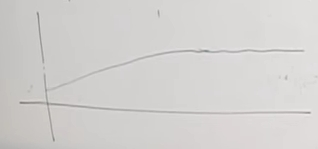
\includegraphics[width=0.9\textwidth]{2proton1ElectronEnergy}\label{fig:2proton1ElectronEnergy}
	\end{subfigure}
	\begin{subfigure}{0.45\textwidth}
		\caption{Electron exchange between protons. This lowers energy, leading to attraction.}
		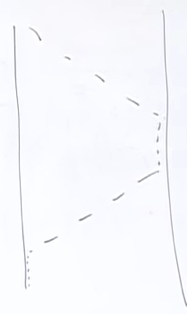
\includegraphics[width=0.9\textwidth]{2proton1ElectronHopping}\label{fig:2proton1ElectronHopping}
	\end{subfigure}
\end{figure}

Key idea: adding wave functions leads to a lower energy state. Energy lowered by alternating between states.

Add 2nd electron, then total charge is zero, giving nett attraction. 

\begin{itemize}
	\item So classically, add 2nd charge, lower energy (creates force) by distorting wave function.
	\item In QM, possibility of swapping between states lowers energy.
\end{itemize}
Can we think of Coulumb force in QM terms? Consider single proton and electron: proton interacts with electromagnetic field, whose quanta are photons.

\begin{itemize}
	\item Classically we solve field equations;
	\item In QM we think of emission and absorption of photons; this is what the Lagrangian tells us. One way to think of this is that the electron is a QM superposition of states: no photons, one with photon emitted,  one with two photons emitted, photon reabsorbed--Figure \ref{fig:2-1-electron-photons}. In Figure \ref{fig:2-1-electron-photons}, when electrons very far apart, energies just add. When they get closer, fields interact, or, in the language of Feynman diagrams, one electron absorbs electron emitted by the other--Figure \ref{fig:2-1-electron-photons-feynmann}.  Energy is no longer sum of energies of individual electrons, which gives rise to Coulomb force.
\end{itemize}

\begin{figure}[H]
	\caption{Emission and absorption of photons}
	\begin{subfigure}{0.45\textwidth}
		\caption{Electron absorbing and reabsorbing photons.}
		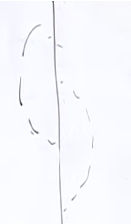
\includegraphics[width=0.9\textwidth]{2-1-electron-photons0}
	\end{subfigure}
	\begin{subfigure}{0.45\textwidth}
		\caption{The electron is a QM superposition of states}\label{fig:2-1-electron-photons}
		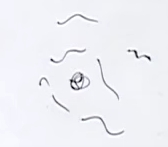
\includegraphics[width=0.9\textwidth]{2-1-electron-photons}
	\end{subfigure}
	\begin{subfigure}{0.45\textwidth}
		\caption{Two Electrons absorbing and reabsorbing photons.}\label{fig:2-1-second-electron-photons}
		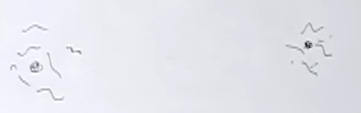
\includegraphics[width=0.9\textwidth]{2-1-second-electron-photons}
	\end{subfigure}
		\begin{subfigure}{0.45\textwidth}
		\caption{Feynman diagram of Electrons absorbing and reabsorbing photons. Sometimes one electron absorbs photon emitted to other.}\label{fig:2-1-electron-photons-feynmann}
		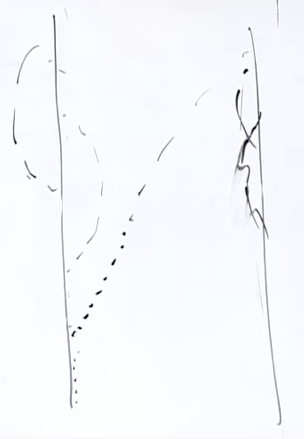
\includegraphics[width=0.9\textwidth]{2-1-second-electron-photons-feynman}
	\end{subfigure}
\end{figure}

In summary we have three ways of looking at forces:

\begin{itemize}
	\item Laws such as Coulomb;
	\item Classical fields theory;
	\item exchange of particles. Every particle can be exchanged, so every particle produces a force. Not just 4 forces! 
\end{itemize}

Standard Model is a mess. We don't understand why the particles are as they are. We understand some relationships. More types of particles than known relationships.

\begin{table}[H]
	\begin{center}
		\caption{Particles (Field symbol)}
		\begin{tabular}{|l|l|l|r|l|r|}\hline
			Name&Symbol&Type&Charge&B\#&Mass\\ \hline
			photon&$\gamma$ A&B&0&0&0 \\ \hline
			electron&$e+\pm \Psi_e\}$&F&-1&0&$0.15MeV$\\ \hline
			Quark&q&F&&$\frac{1}{3}$&\\ \hline
			down&q(Q) $\Psi_q$&F&$-\frac{1}{3}$&$\frac{1}{3}$&10meV\\ \hline
			up&&F&$\frac{2}{3}$&$\frac{1}{3}$&5meV\\ \hline
			strange&&F&$-\frac{1}{3}$&$\frac{1}{3}$&100meV\\ \hline
			charm&&F&$\frac{2}{3}$&$\frac{1}{3}$&1GeV\\ \hline
			bottom&&F&$-\frac{1}{3}$&$\frac{1}{3}$&5Gev\\ \hline
			top&&F&$\frac{2}{3}$&$\frac{1}{3}$&170Gev\\ \hline
			&&&&&\\ \hline
			&&&&&\\ \hline
		\end{tabular}
	\end{center}
\end{table}

\begin{enumerate}
	\item Particle and Field usually have the same name
	\item charge--electron is unit
	\item eV
	\item Proton has Baryon number 1.
	\item 3 families of quarks. Why?
\end{enumerate}

Figure \ref{table:mesons} depicts the way that electromagnetic processes emerge from a Lagrangian.

\begin{figure}[H]
	\caption{$\mathcal{L}$: $e \Psi_e^\dagger \Psi_e A$}\label{fig:fep}
	\begin{subfigure}{0.45\textwidth}
		\caption{Fundamental electromagnetic process. Can rearrange.}\label{fig:fep1}
		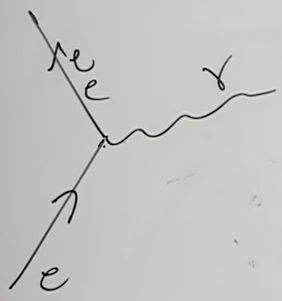
\includegraphics[width=0.9\textwidth]{2-1-em-process}
	\end{subfigure}
	\begin{subfigure}{0.45\textwidth}
		\caption{Fundamental electromagnetic process--exchange of particle.}\label{fig:fep2}
		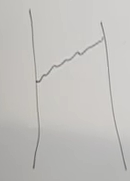
\includegraphics[width=0.9\textwidth]{2-1-em-process-feynman}
	\end{subfigure}
\end{figure}

Three quarks build baryons, two mesons--Table \ref{table:mesons}.
\begin{itemize}
	\item neutron: ddu (slightly heavier)
	\item proton: uud (self energy of energy partially offsets difference in quark masses)
\end{itemize}

Can we make an analogue of proton/neutron with strange quarks? Yes. E.g. sdu, ssu, uus -- Strange baryons.


\begin{table}[H]
	\begin{center}
		\caption[Mesons: baryon number 0 - quark + anti-quark]{Mesons: baryon number 0 - quark + anti-quark. Note the two entangled pairs: $\frac{1}{\sqrt{2}}\big(\ket{\bar{u}u}\pm\ket{\bar{d}d}\big)$}\label{table:mesons}
		\begin{tabular}{|l|l|l|r|} \hline
			&Quarks&Charge&Mass\\ \hline
			$\pi^-$&$\bar{u}d$&-1&$\approx140 meV$ \\ \hline
			$\pi^+$&$u\bar{d}$&+1&$\approx140 meV$  \\ \hline
			$\pi^0$&$\frac{1}{\sqrt{2}}\big(\ket{\bar{u}u}+\ket{\bar{d}d}\big)$&0&$\approx140 meV$  \\ \hline
			$\eta$&$\frac{1}{\sqrt{2}}\big(\ket{\bar{u}u}-\ket{\bar{d}d}\big)$& 0&$\approx500 meV$ \\ \hline
			&$\bar{u}s$&-1& \\ \hline
			&$u\bar{s}$&+1& \\ \hline
			&$\bar{d}s$&0& \\ \hline
			&$d\bar{s}$&0& \\ \hline
			&$\bar{s}s$&0& \\ \hline
		\end{tabular}
	\end{center}
\end{table}

We also have strange mesons ($K-mesans$).


\section{Quantum chromodynamics}

This is the theory of Quarks and gluons, and the things that they make.

\begin{defn}[Hadron]
	The things that Quarks and gluons make are called hadrons.
\end{defn}

\begin{defn}[Baryon]
	Things made from 3 quarks are called baryons.
\end{defn}

\begin{defn}[Meson]
	Mesons are quark-anti-quark pairs.
\end{defn}

\begin{defn}[Gluon]
	Electrically neutral stuff than holds quarks and antiquarks together.
\end{defn}

Spin without group theory. We start with the basic commutation relations:\cite{susskind2009particles}
\begin{align*}
	[L_x,L_y] =& i \hslash L_z\\
	[L_y,L_z] =& i \hslash L_x\\
	[L_z,L_x] =& i \hslash L_y
\end{align*}

In \cite{susskind2009particles}:

\begin{itemize}
	\item We broke the symmetry by focusing on $L_z$.
	\item We can measure only one $L_i$ at a time.
	\item $L_i$ is quantized--$\hslash$.
\end{itemize}

\begin{table}[H]
	\begin{center}
		\caption{Spin multiplets: Spin $l$ denotes highest $L_z$.}
		\begin{tabular}{|c|c|l|} \hline
		$l$&Range of $L_z (Number=2l+1)$&Statistics\\ \hline
		$0$&$0$& Boson\\ \hline
		$\frac{1}{2}$&$\{-\frac{1}{2},\frac{1}{2}\}$& Fermion\\ \hline
		$1$&$\{-1,0,1\}$&Boson \\ \hline
		$\frac{3}{2}$&$\{-\frac{3}{2},-\frac{1}{2},\frac{1}{2},\frac{3}{2}\}$&Fermion \\ \hline
		$2$&$\{-2,-1,0,1,2\}$&Boson \\ \hline
		\end{tabular}
	\end{center}
\end{table}

\begin{table}[H]
	\begin{center}
		\caption[Ways to put two spin $\frac{1}{2}$ particles together]{Ways to put two spin $\frac{1}{2}$ particles together. Consider whether particles could disappear with violating conservation of angular momentum.}
		\begin{tabular}{|l|l|l|l|}\hline
			&$l$&$L_z$&Could disappear?\\ \hline
			$\ket{\uparrow\uparrow}$ &1&1&no--has $L_z$\\ \hline
			$\ket{\downarrow\downarrow}$&1&-1&no--has $L_z$ \\ \hline
			$\frac{1}{\sqrt{2}}(\ket{\uparrow\downarrow}+\ket{\downarrow\uparrow})$ &1&0&no--has $L_x$\\ \hline
			$\frac{1}{\sqrt{2}}(\ket{\uparrow\downarrow}-\ket{\downarrow\uparrow})$ &0&0&yes\\ \hline
		\end{tabular}
	\end{center}
\end{table}


\begin{table}[H]
	\begin{center}
		\caption{$3 \times \frac{3}{2}$ spins.}
		\begin{tabular}{|l|r|c|}\hline
			$\ket{\uparrow\uparrow\uparrow}$&$\frac{3}{2}$& \\ \hline
			$\ket{\downarrow\downarrow\downarrow}$&$-\frac{3}{2}$& \\ \hline
			$\ket{\uparrow\downarrow\downarrow}$,$\ket{\downarrow\uparrow\downarrow}$,$\ket{\downarrow\downarrow\uparrow}$&$\frac{1}{2}$&Three ways to do this\\ \hline
			$\ket{\uparrow\downarrow\downarrow}$,$\ket{\downarrow\uparrow\downarrow}$,$\ket{\downarrow\downarrow\uparrow}$&$-\frac{1}{2}$&Three ways to do this\\ \hline
		\end{tabular}
	\end{center}
\end{table}

\subsection{Isospin}

Natural energy of nucleus is a few hundred meV: up and down quarks. To a first approximation, masses are closer to each other, so they are analogous to spin. Thinking of up and down quarks as isomorphic to up and down spins, we invent the concept of iso spin.

\begin{itemize}
	\item $(\uparrow,\downarrow)$ Spin
	\item $(u,d)$ Isospin i.e.  $(p,n)$--makes Isotope.
\end{itemize}

Isospin isn't a precise symmetry of nature, as $u$ and $d$ have different masses and charges. But is is an approximate symmetry, for strong forces only.

Simplest object we can study is 3 quarks. We can make an object of isotopic spin $\frac{1}{2}$ or $\frac{3}{2}$--Table \ref{table:3quark}.

\begin{itemize}
	\item Assume that we can label quarks--${1,2,3}$
	\item Quarks are Fermions, so we need to anti-symmetrize. For example the proton should be: $\underbrace{d_1}_\text{isospin $\frac{1}{2}$}\underbrace{(u_2u_3-u_3u_2)}_\text{isospin 0}$.
	\item $\frac{1}{2}$: two states (isotopic spin doublet)
	\item $\frac{3}{2}$. $uuu$ and $ddd$, $\uparrow\uparrow\uparrow$, $\downarrow\downarrow\downarrow$. There are 4 states for isospin $\frac{3}{2}$--an isospin multiplet. NB, this $\Delta_\frac{3}{2}$ differs from the nucleon, as all spins are aligned. The $uud$ and $uud$ have an isospin component of $\frac{1}{2}$, even though total isotopic spin is $\frac{3}{2}$.
\end{itemize}

\begin{table}[H]
	\begin{center}
		\caption[Simplest object we can study is 3 quarks.]{Simplest object we can study is 3 quarks. We can make an object of isotopic spin $\frac{1}{2}$ or $\frac{3}{2}$.}\label{table:3quark}
		\begin{tabular}{|c|c|c|c|r|r|}\hline
			Isospin&Quarks&Spin&Name&Charge&Mass\\ \hline
			$\frac{1}{2}$&-$d_1u_2u_3$&$\frac{1}{2}$&proton&$+1$&940meV\\ \hline
			$\frac{1}{2}$&$u(dd)$&$\frac{1}{2}$&neutron&0&940meV\\ \hline
			$\frac{3}{2}$&uuu&$\frac{3}{2}$&$\Delta_\frac{3}{2}$&$+2$&1200meV\\ \hline
			$\frac{3}{2}$&ddd&$\frac{3}{2}$&$\Delta_\frac{3}{2}$&-1&1200meV\\ \hline
			$\frac{3}{2}$&uud&$\frac{3}{2}$&$\Delta_\frac{3}{2}$&+1&1200meV\\ \hline
			$\frac{3}{2}$&udd&$\frac{3}{2}$&$\Delta_\frac{3}{2}$&0&1200meV\\ \hline
		\end{tabular}
	\end{center}
\end{table}

Figure \ref{fig:decay:dalta} shows that $\Delta_\frac{3}{2}$ decays.

\begin{figure}[H]
	\begin{center}
		\caption[Decay of a $\Delta_\frac{3}{2}$]{Decay of a $\Delta_\frac{3}{2}$. Quarks can't go off on their own, so we need a quark-antiquark pair to balance. $\Delta_\frac{3}{2}\rightarrow p +\pi^+$: there is enough energy left.}\label{fig:decay:dalta}
		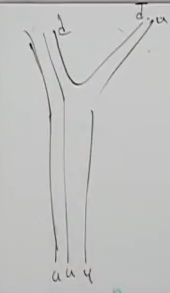
\includegraphics[width=0.6\textwidth]{2-2-Delta-decay}
	\end{center}
\end{figure}

\subsection{Quantum chromodynamics}

We have a problem: $uuu$ represents three Fermions shose spins are all in the same direction! This violates the Pauli Exclusion Principle. Quarks must have another property, so the three quarks must have a label which is hidden from view and not apparent in experiments. This is called "colour", a totally arbitrary name which has nothing to do with ordinary colour: it is just a name. Values are Red, Blue, and Green. The important thing is that they have precisely 3 different values. The  $\Delta_\frac{3}{2}$ is important because of having 3 u or d. For proton we need to symmetrize:$\ket{d_R u_G u_B}+...$

What holds quarks together? Electrons use protons / electromagnet field. Quarks use gluons: spin 1, so same polarization states, massless, but one big difference(later), and they jump back and forth. Quarks emit and absorb gluons.

The fundamental electromagnetic process is depicted in Figure \ref{fig:fep1}. A photon is similar to electron and positron, e.g. it has the same properties: a sufficiently energetic photon can decay into an electron and positron pair.

\begin{figure}[H]
	\caption{Gluons}
	\begin{subfigure}{0.45\textwidth}
		\caption{Introducing the gluon}
		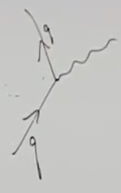
\includegraphics[width=0.9\textwidth]{2-2-gluon1}
	\end{subfigure}
	\begin{subfigure}{0.45\textwidth}
		\caption{A gluon behaves a bit like a quark-antiquark pair: this the gluon as a fictitious quark-antiquark pair}
		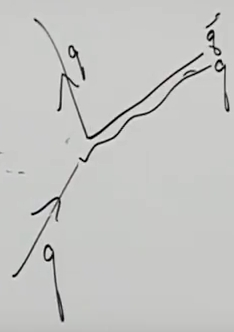
\includegraphics[width=0.9\textwidth]{2-2-gluon2}
	\end{subfigure}

\end{figure}

There are 9 possible gluons (we will see later that there are actually only 8):
\begin{align*}
\begin{pmatrix}
R\bar{R}&R\bar{G}&R\bar{B}\\
G\bar{R}&G\bar{G}&G\bar{B}\\
B\bar{R}&B\bar{G}&B\bar{B}
\end{pmatrix}
\end{align*}

Gluons can interact with each other--Figure \ref{2-2-gluon6}.
\begin{figure}[H]
	\caption{The basic vertices of QCD}
	\begin{subfigure}{0.45\textwidth}
		\caption{Red quark changes to green: analogous to process with photon.}
		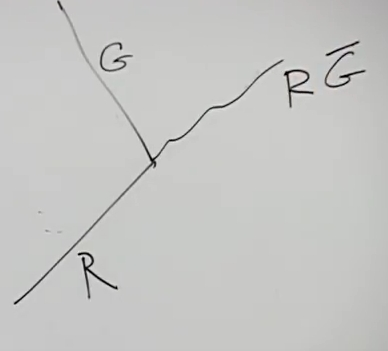
\includegraphics[width=0.9\textwidth]{2-2-gluon3}
	\end{subfigure}
	\begin{subfigure}{0.45\textwidth}
		\caption{Red quark changes to green, using fictitious quark-antiquark pair}
		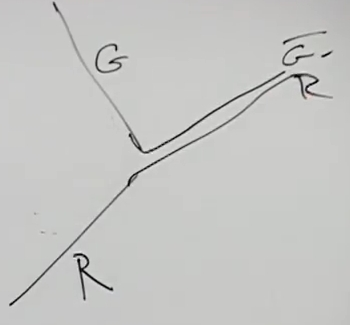
\includegraphics[width=0.9\textwidth]{2-2-gluon4}
	\end{subfigure}
	\begin{subfigure}{0.45\textwidth}
		\caption{Second basic vertex, which has no analogue for photons. Fictitious quark-antiquark pairs represent gluons. This process makes QCD more complex and more interesting.}\label{2-2-gluon5}
		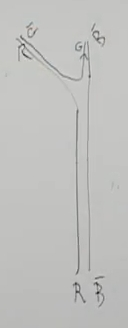
\includegraphics[width=0.9\textwidth]{2-2-gluon5}
	\end{subfigure}
	\begin{subfigure}{0.45\textwidth}
		\caption{Second basic vertex, redrawn with gluons, instead of fictitious quark-antiquark pairs. Use Figure \ref{2-2-gluon5} to determine which combinations don't break any lines.}\label{2-2-gluon6}
		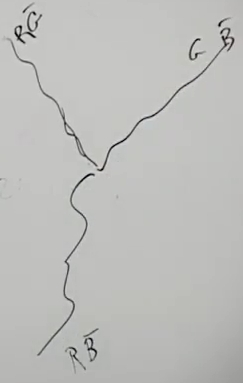
\includegraphics[width=0.9\textwidth]{2-2-gluon6}
	\end{subfigure}
\end{figure}

Forces. Photons cannot exchange photons, but gluons can exchange gluons, which means that there are forces between gluons--Figure \ref{fig:quarks:gluons:forces}. Two waves of gluons can deform each other; different parts of one wave of gluons can deform each other. Dynamics is non-linear.

\begin{figure}[H]
	\caption{Photons cannot exchange photons, but gluons can exchange gluons.}\label{fig:quarks:gluons:forces}
	\begin{subfigure}{0.45\textwidth}
		\caption{Force between quarks}
		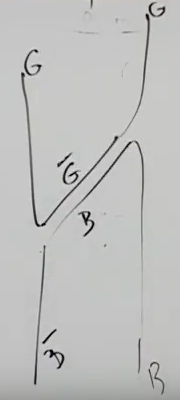
\includegraphics[width=0.9\textwidth]{2-2-gluon7}
	\end{subfigure}
		\begin{subfigure}{0.45\textwidth}
		\caption{Force between gluons}
		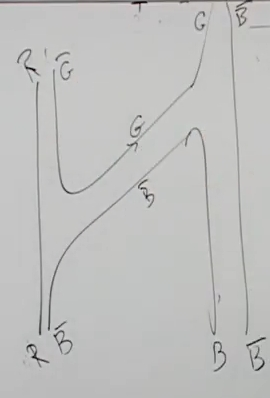
\includegraphics[width=0.9\textwidth]{2-2-gluon8}
	\end{subfigure}
\end{figure}

The only rule is: follow the lines and, if the line turn around, change to antiparticle.

\begin{itemize}
	\item Move gradually - whole thing
	\item Move at high frequency, m only
\end{itemize}

Figure \ref{fig:2-2-mass1} shows that masses of objects are frequency dependent. In the same sense, masses of quarks depend on frequency. Move slowly and we drag gluons. High frequency get mass of quark. Concept of mass of quark is ambiguous: normally use high frequency mass
\begin{figure}[H]
	\caption[Mass with squishy thing attached]{Mass with squishy thing attached. If we move slowly we drag attachment, fast we just move mass.}\label{fig:2-2-mass1}
	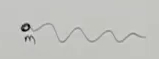
\includegraphics[width=0.8\textwidth]{2-2-mass1}
\end{figure}


\section{Group theory I}

Rotations in space act on vectors: they rotate one vector to another. Rotations can be combined: they form a non-Abelian group. Figure \ref{fig:2-3-paramerize-rotation} depicts one way to parametrize rotation--axis $\vec{n}$ and angle $\theta$. Since $\vec{n}$ can be parametrized by two angles, latitude and longitude, we need 3 angles in total.

\begin{figure}[H]
	\caption{Paramerize rotation: axis $\vec{n}$ and angle $\theta$}\label{fig:2-3-paramerize-rotation}
	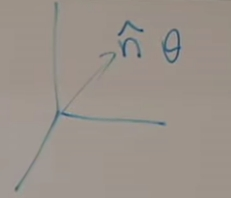
\includegraphics[width=0.8\textwidth]{2-3-paramerize-rotation}
\end{figure}

Representations. Colour is representation of the rotation group.

How do we construct a matrix representation of rotations? WE consider the 3D representation of the 3D rotation group.
\begin{align*}
\sum_j R_{ij}(\theta,\vec{n})V_j=&V_i^\prime \\
R \vec{V} =&\vec{V^\prime} \text{. Now if $R$ is a rotation, it doesn't change length}\\
\forall \vec{V} \; \sum_i V_i^2 =& \sum_i (V_i^\prime)^2\\
\sum_{i,j,k} R_{ij} R_{ik} V_j V_k =& \sum_i V_i V_i \text{, i.e.}\\
\sum_{i} R_{ij} R_{ik} =& \delta_{j,k} \text{, or}\\
R^T R =& I
\end{align*}

There are 3D representations of the rotation group. Can we think of them being related to quantum states? Spin describes angular momentum. A spin 1 particle (vector boson) can be described by a column vector containing amplitudes for the various components of spin. What about spin $\frac{1}{2}$ particle?

\begin{align*}
	\begin{pmatrix}
		1\\
		0
	\end{pmatrix}=& \ket{u}\\
	\begin{pmatrix}
		0\\
		1
	\end{pmatrix}=& \ket{d}\\
	\begin{pmatrix}
		\alpha_1\\
		\alpha_2
	\end{pmatrix}=& \alpha_1 \ket{u} + \alpha_2 \ket{v} \text{, where $\alpha_1^2+\alpha_2^2=1$}
\end{align*}

We can represent rotation by a $2\times2$ matrix acting on spinors.

\begin{align*}
	\begin{pmatrix}
		U_{11}&U_{12}\\
		U_{21}&U_{22}
	\end{pmatrix} 	\begin{pmatrix}
		\alpha_1\\
		\alpha_2
	\end{pmatrix} =& \begin{pmatrix}
		\alpha^\prime_1\\
		\alpha^\prime_2
	\end{pmatrix} \text{{. Now if}}\\
	\alpha^*_1 \alpha_1 + \alpha^*_2 \alpha_2 =& 1 \text{ we want}\\
	(\alpha^\prime_1)^* (\alpha^\prime_1) + (\alpha^\prime_2)^* (\alpha^\prime_2) =& 1 {, which gives}\\
	(U^T)^* U =& I \text{, which can be written} \\
	U^\dagger U =& I \numberthis \label{eq:unitary:2}
\end{align*}

U has 8 degrees of freedom, but (\ref{eq:unitary:2}) imposes 4 constraints, yielding 4 degrees of freedom. But 3D rotations only have 3 degrees of freedom. We set $\det(U)=1$ to give a 3 parameter group, $SU(2)$

\begin{defn}[$U(N)$]
	The group of unitary $N\times N$ matrices.
\end{defn}

\begin{defn}[$SU(N)$]
	The group of unitary $N\times N$ matrices with determinant 1.
\end{defn}

For small rotations:
\begin{align*}
	U =& I + i \epsilon M \\
	I =&U U^\dagger\\
	 =& (I + i \epsilon M)(I - i\epsilon M^\dagger)\\
	 =& I + i \epsilon(M - M^\dagger) - \epsilon^2 M^\dagger \text{, whence, discarding $\epsilon^2$}\\
	 M - M^\dagger =& 0 \text{. We also need U to be unimodular}\\
	1=&\det(U)\\
	 =& \det( I + i \epsilon M)\\
	=& 1 + i\epsilon(Tr(M)) \text{, whence:}\\
	Tr(M) =&0
\end{align*}
But any traceless Hermitian $2\times2$ matrix can be written as a linear combination of the Pauli  matrices $\sigma_i$:
\begin{align*}
	\sigma_x =& \begin{pmatrix} \numberthis \label{eq:pauli:x}
		0&1\\
		1&0
	\end{pmatrix}\\
	\sigma_y =& \begin{pmatrix} \numberthis \label{eq:pauli:y}
		0&-i\\
		i&0
	\end{pmatrix}\\
	\sigma_z =& \begin{pmatrix} \numberthis \label{eq:pauli:z}
		1&0\\
		0&-1
	\end{pmatrix}
\end{align*}

State of quark can be Red, Green, or Blue. 
\begin{align*}
	\begin{pmatrix}
		\alpha_1\\
		\alpha_2\\
		\alpha_3
	\end{pmatrix} \quad	\begin{pmatrix}
	\Psi_r\\
	\Psi_g\\
	\Psi_b
	\end{pmatrix}
\end{align*}

We can multiply by a member of $SU(3)$. These have $18-9-1=8$ degrees of freedom. Every term in Lagrangian needs to be invariant under $SU(3)$.  


\section{Group theory – II}

$SU(2)$ is not exactly the same as 1D rotations: there is a $2\rightarrow1$ correspondence, not  $1\rightarrow1$, since $-U$ and $U$ correspond to the same rotation. This is why the electron wave function is called a doublet.

Generators are closely connected to infinitesimal elements. If you know structure of generators you can work out the whole structure. Generators let us figure out conservation laws.

\begin{align*}
	U =& I + i \epsilon T\\
	I =& U^\dagger U + 1\\
	=& I + i\epsilon(T - T^\dagger) - \epsilon^2 T T^\dagger\\
	T =& T^\dagger \text{. Hermitian -- observable}\\
	\det(U) =& 1\\
	\implies&\\
	Tr(t)=&0
\end{align*}

Since the rotation group has three parameters, the Ts span a 3D space. See (\ref{eq:pauli:x}), (\ref{eq:pauli:y}), and (\ref{eq:pauli:z}). Can figure out generators from commutation rules.

In SU(3) we have $3\times3$ matrices, so $3\times3\times2=18$ real components; the matrix being unitary imposes 9 constraints, and unimodularity imposes one more, whence there are $18-9-1=8$ degrees of freedom.

Combining representations to form new representations. E.g. we might compose spins to make a composite. E.g. combine 2 spin $\frac{1}{2}$ objects. We have 4 possible states: a basis in that space can be thought of as a spin 0 object plus 3 spin 1 objects. We can make ${-1,0,+1}$, but the zero can be done in 2 ways: so one of the zero spins must not be part of the spin 1 multiplet, it can only be spin 0 (ortho- and para-hydrogen).

Representations of $SU(3)$.

Triplet: $3\times3$ matrix acting on RGB vector, mixing up states, transforming to a quantum superposition.

There are 3 important representations:

\subsubsection{3 ("the 3")}

\begin{align*}
	\begin{pmatrix}
		q_r\\
		q_g\\
		q_b
	\end{pmatrix} \text{ field operator--creation}
\end{align*} 

\subsubsection{$\bar{3}$}

Antiquarks, represented by complex conjugates (not Hermitian conjugates)/

\begin{align*}
	U q =& q^\prime\\
	U^* q^* = q^\prime& 
\end{align*}

Electron and positron are complex conjugate representations of $U(1)$. ($e^{i\theta}\psi_e \rightarrow e^{-i\theta}\psi_p$).

Generators of $\bar{3}$ are negatives of generators of $3$, so they carry negative colour.

\subsubsection{$3 \otimes 3$}

Combine two quarks ${RR, RG, RB,...}$

\begin{align*}
	3 \otimes 3 =& \underbrace{\bar{3}}_\text{combine antisymmetrically} \oplus \underbrace{6}_\text{combine symmetrically}\\
	3 \otimes \bar{3} =& \underbrace{1}_\text{singlet: $R\bar{R}+G\bar{G}+B\bar{B}$} \oplus \underbrace{8}_\text{8 dimensional representation--generators!}
\end{align*}

\begin{align*}
3 \otimes 3 \otimes 3 =& (3 \otimes 3) \otimes 3\\
=& \big(\bar{3} \oplus 6 \big) \otimes 3\\
=& \bar{3}   \otimes 3 + 6 \otimes 3\\
=& \underbrace{1}_\text{anti-symmetrized superposed R, B, B} \oplus 8 \oplus 8 \oplus 10
\end{align*}

Gluon behaves a quark-antiquark under colour symmetry: it transforms under the 8 (octet).

\url{https://youtu.be/n88Qe-aAAYE?t=2883}


\section{Gauge fields and symmetry}

TBP

\section{The weak interaction}

TBP

\section{Spontaneous symmetry breaking and Goldstone bosons}

TBP

\section{The Higgs field}

TBP

\section{The Higgs field and fermions}

TBP

\section{Renormalization and the running of coupling constants}

TBP

\begin{appendices}
	\section{Demystifying the Higgs Boson}
	\cite{susskind2010demystifing}
	TBP
\end{appendices}

\bibliographystyle{unsrt}
\addcontentsline{toc}{section}{Bibliography}
\raggedright
\bibliography{tm}


\end{document}
